\section{Задание}

\subsection{Вариант 4}

\begin{enumerate}
    \item Исследовать влияние уровня автоматизации процесса разработки на трудоемкость (РМ) и время разработки проекта (ТМ) для модели COCOMO и разных типов проектов (обычного, промежуточного, встроенного). Получить значения PM и ТМ по всем типам проектов для одного и того же значения параметра размера программного кода (SIZE), выбрав номинальный, низкий и высокий уровень использования современных методов и программных инструментов. Результаты исследований оформить графически.

    \item Компания получила заказ на разработку программного обеспечения для рабочей станции дизайнера автомобиля. Заказчик следующим образом определил проблемную область в своей спецификации: ПО должно формировать 2-х и 3-х мерные изображения для дизайнера, система должна иметь стандартизованный графический интерфейс, геометрические и прикладные данные должны содержаться в базе данных (планируемый размер базы данных не более 200 тыс. записей). При анализе проекта его размер был предварительно оценен в 140 000 строк кода. Проект реализуется по промежуточному варианту. Все показатели драйверов затрат, кроме трех имеют номинальное значение. Знание языка программирования имеет высокую оценку, использование современных методов – очень высокую оценку и использование программных инструментов – низкую, так как используется стандартная среда визуального программирования. Произвести оценку показателей проекта по методике СОСОМО.
\end{enumerate}

\section{Задание 1}

Было произведено исследование зависимости значения трудозатрат от уровня использования современных методов (параметр MODP) при очень низкой и очень высокой сложности продукта (параметр CPLX).

\begin{figure}[H]
	\centering
	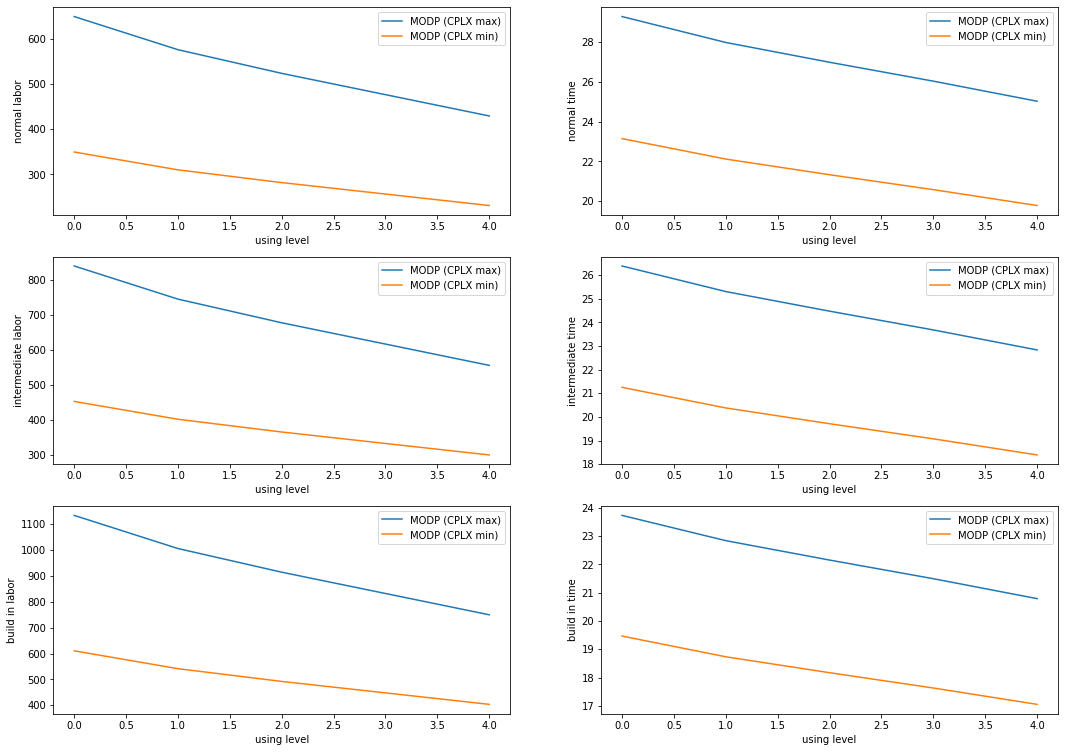
\includegraphics[width=0.8\textwidth]{img/content/task_01.png}
	\caption{Графики}
	\label{fig:task_01}
\end{figure}

На графиках видно, что чем выше значимость параметра MODP, тем ниже трудозатраты и время выполнения проекта. Также видно, что при повышении сложности проекта оба параметра тоже повышаются.

\section{Задание 2}

В соотвествии с 4 вариантом задания, были рассчитаты параметры трудозатрат и времени данного проекта.

\begin{figure}[H]
	\centering
	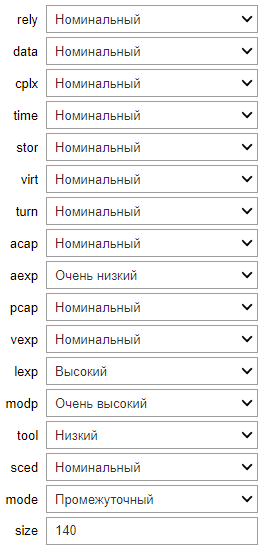
\includegraphics[width=0.3\textwidth]{img/content/task_02_params.png}
	\caption{Входные параметры проекта}
	\label{fig:task_02_params}
\end{figure}

\begin{figure}[H]
	\centering
	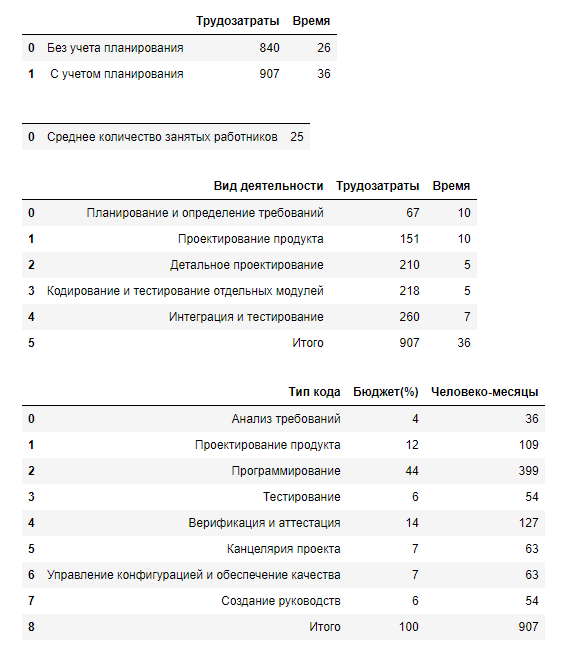
\includegraphics[width=0.7\textwidth]{img/content/task_02_result.png}
	\caption{Результаты}
	\label{fig:task_02_result}
\end{figure}

\begin{figure}[H]
	\centering
	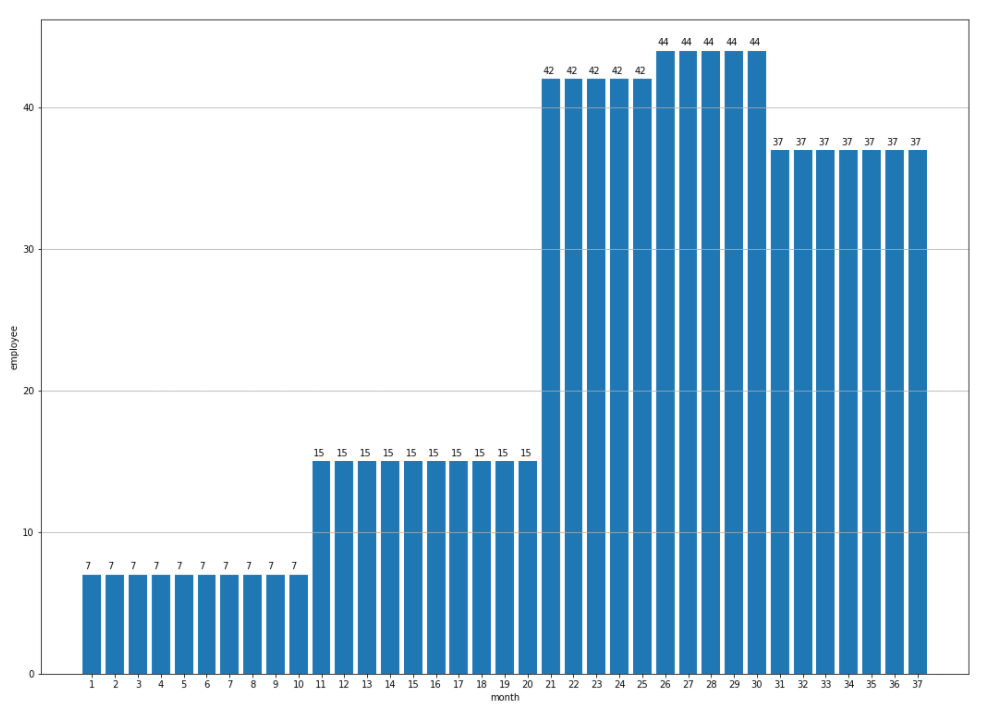
\includegraphics[width=0.8\textwidth]{img/content/task_02_plot.png}
	\caption{Диаграмма привлечения сотрудников}
	\label{fig:task_02_plot}
\end{figure}

В качестве средней зарплаты было взято значение 130'000 рублей. С таким значением заработной платы бюджет составил 127'342'800 рублей.

\section{Вывод}

Использование метода COCOMO действительно позволяет дать первичную оценку проекта, используя только знания о количестве строк кода. Но стоит учитывать, что уже существует COCOMO 2, которая может учесть такие моменты как: <<ПО должно формировать 2-х и 3-х мерные изображения для дизайнера, система должна иметь стандартизованный графический интерфейс>>, и вполне возможно способна дать более высокую точность ответа на вопрос о колтчестве трудозатрат и времени разработки проекта. Тем ни менее, в рамках данного проекта мы все таки смогли получить первичные знания используя COCOMO 1.

